\chapter{Estimation de la réponse fréquentielle du canal de propagation dans les structures d'égalisation DFVE}

\paragraph{}
Dans ce chapitre, nous supposons ne plus connaître la réponse fréquentielle du
canal, et donc nous ne connaissons plus les matrices qui interviennent dans les
structures d'égalisation DFVE. Le but est de les approcher grâce au principe de
l'algorithme LMS (Algorithme du gradient stochastiques).

\section{Création du signal et modélisation du canal de propagation}
\paragraph{}
Dans notre signal, nous avons ajouté des pilotes. Les pilotes sont des états
connus qui servent à estimer le canal à la réception. Dans notre cas, l'état des
pilotes a été pris à $1+j$, et ces pilotes ont été inséré tout les 3 symboles
OFDM, sur nos 4 porteuses. Figure ~\ref{etatavecpilotes}, nous pouvons voir le
signal que nous voulons envoyer après modulation $\pi/4$-QPSK avec les pilotes.
\paragraph{}
\vspace{1\baselineskip}
\begin{figure}[!h]
  \centering
  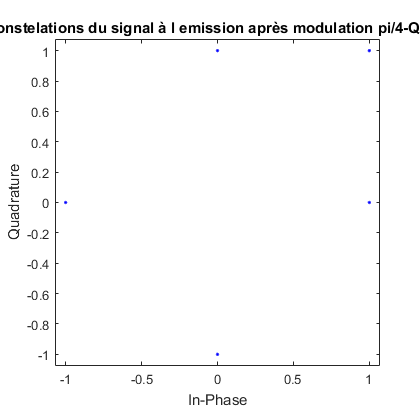
\includegraphics[scale=0.6]{emissionavecpilote.png}
  \caption{Signal après modulation QPSK et avec ajout des pilotes }
	\label{etatavecpilotes}
\end{figure}
\vspace{10\baselineskip}

\paragraph{}
Le canal de propagation fût modélisé comme dans le chapitre précédent, et Figure
~\ref{sanstraitement}, on peut voir le signal reçu à la réception avant les
traitements.
\paragraph{}
\vspace{1\baselineskip}
\begin{figure}[!h]
  \centering
  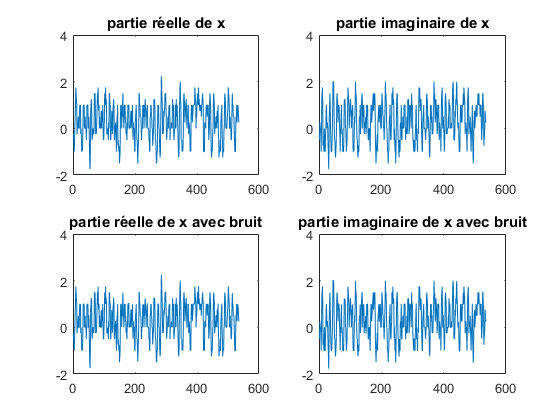
\includegraphics[scale=0.7]{sanstraitement.png}
  \caption{Signal reçu par le récepteur}
	\label{sanstraitement}
\end{figure}
\vspace{2\baselineskip}


\section{Égalisation avec estimation de la réponse du canal}

\paragraph{}
Dans les deux structures, il faut un point de départ pour les matrices. Pour
simuler la convergence vers nos bonnes matrices, nous avons fausser celle de
départ en ajoutant des valeurs aux coefficients de $H_0$ et de $H_1$. De plus,
nous avons un pas d'adaptation $\mu$ de 0.01. De notre interprétation, le pas
d'adaptation petit ralentit l'estimation de la réponse du canal, mais on sera
plus précis. Si notre pas est grand, on sera rapide, mais moins précis.

\subsection{Structure fréquentielle d'égalisation DFVE}
\paragraph{}
Dans notre chaîne de réception, lors de la réception de nos pilotes, nous
ré-estimons nos matrices $P_0$ et $P_1$ avec les formules 12a et 12b de
\cite{sujet}. Une fois les états du signal estimés, nous enlevons les pilotes,
et nous obtenons le diagramme de constellation visible sur la Figure
~\ref{etatsanspilote}.

\paragraph{}
\vspace{1\baselineskip}
\begin{figure}[!h]
  \centering
  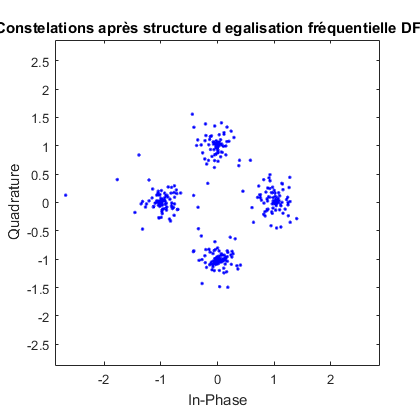
\includegraphics[scale=0.6]{etatsanspilotes.png}
  \caption{États du signal estimés après extraction des pilotes dans la structure fréquentielle }
	\label{etatsanspilote}
\end{figure}

\paragraph{}
Après comparaison avec le signal émis, nous obtenons 0\% d'erreurs sur l'ensemble du signal.


\subsection{Structure temporelle d'égalisation DFVE}

\paragraph{}
Pour la structure temporelle, on estime $Q_0$ et $Q_1$ dans la boucle, mais on
fait une estimation sous optimale sur $Q_1$ afin de réduire la complexité. A
cause de cette estimation, nous avons toujours plus d'erreurs que dans la
structure fréquentielle, comme 1.12\% où l'on trouvait 0\% pour la structure
fréquentielle.
\paragraph{}
Afin de mieux illustrer le signal après estimation, nous pouvons voir sur la
Figure ~\ref{avecPilote} l'estimation des états par la structure temporelle,
avant extraction des pilotes.
\paragraph{}
\paragraph{}
\vspace{1\baselineskip}
\begin{figure}[!h]
  \centering
  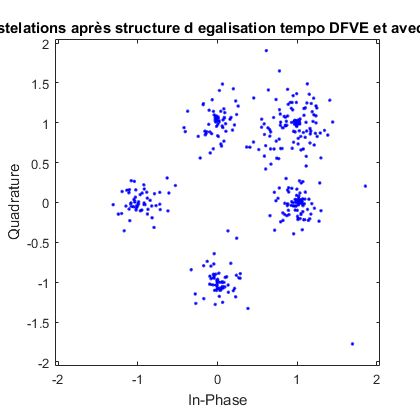
\includegraphics[scale=0.6]{avecPilote.png}
  \caption{États du signal estimés dans la structure temporelle avant extraction des pilotes }
	\label{avecPilote}
\end{figure}
\vspace{1\baselineskip}
\paragraph{}
Afin de tester la convergence de notre méthode, nous avons testé un code où nous
n'ajoutons pas de bruit complexe dans le canal. Nous mettons beaucoup d'erreurs
dans les matrices $H_0$ et $H_1$ initiales, donc dans $Q_0$, $Q_1$, $P_0$ et
$P_1$. Dans un premier test, nous gardons ces matrices, et donc nous ne régulons
pas l'estimation du canal. Nous obtenons 26\% d'erreurs dans les deux
structures. Ensuite nous relançons l'algorithme avec l'estimation continue des
matrices. Nous avons 19\% d'erreurs sur la structure fréquentielle, et 20\% sur
la structure temporelle. C'est normal d'avoir un fort taux d'erreurs ici, car il
faut du temps pour que le récepteur converge vers la bonne estimation. Ce qui est
important ici est d'observer une  meilleure convergence vers
la solution par l'algorithme LMS, car on fini par bien estimer notre
canal. C'est ce que l'on peut voir sur la Figure ~\ref{convergence}. On commence
par des estimations erronées, et à la fin, on peut voir la convergence vers les
bons états.
\paragraph{}
\vspace{1\baselineskip}
\begin{figure}[!h]
  \centering
  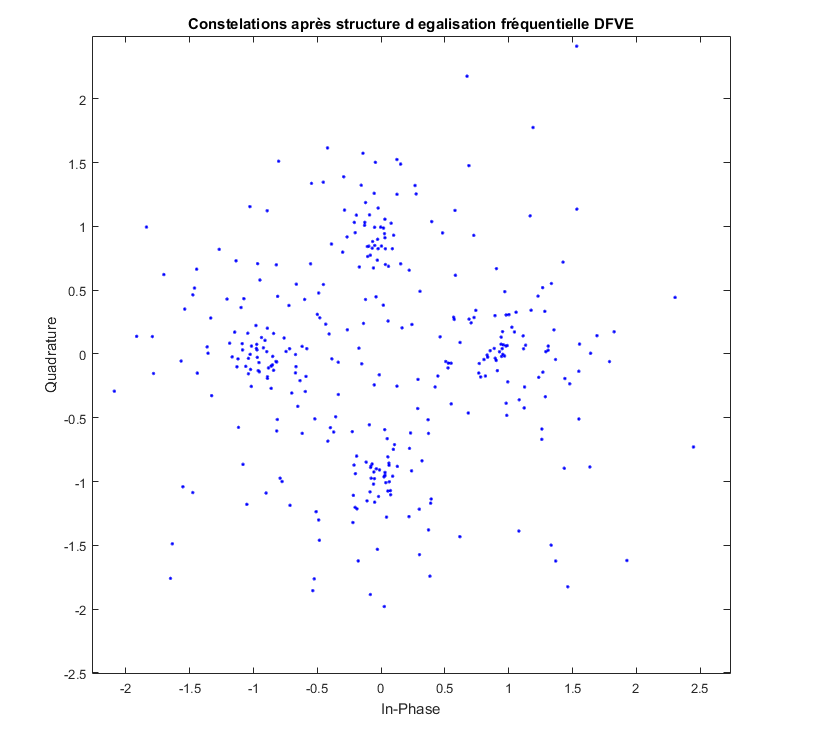
\includegraphics[scale=0.5]{convergence.png}
  \caption{Convergence vers les bons états grâce à l'algorithme LMS }
	\label{convergence}
\end{figure}
\paragraph{}
Nous venons de tester les estimations de la réponse du canal de propagation à
travers les estimations de matrices. Nous avons constaté un compromis entre
complexité de calcul et l'efficacité de l'estimation. En effet, la structure
temporelle diminue fortement la complexité calculatoire, mais il y a plus
d'approximation dans l'estimation du canal, ce qui nous fait perdre de
l'efficacité dans l'estimation final du signal émis. Il faut donc trouver un
juste milieu dans ce que l'on peut corriger grâce à un codage canal, et la
puissance et le temps de calcul minimum.

%%% Local Variables:
%%% mode: latex
%%% TeX-master: "../rapport_de_base"
%%% End:
